\documentclass[
  bibliography=totoc,     % Literatur im Inhaltsverzeichnis
  captions=tableheading,  % Tabellenüberschriften
  titlepage=firstiscover, % Titelseite ist Deckblatt
]{scrartcl}

\usepackage{fixltx2e}
\usepackage[aux]{rerunfilecheck}

\usepackage{polyglossia}
\setmainlanguage{german}

\usepackage{amsmath}
\usepackage{amssymb}
\usepackage{mathtools}

\usepackage{fontspec}
\defaultfontfeatures{Ligatures=TeX}

\usepackage[
  math-style=ISO,
  bold-style=ISO,
  sans-style=italic,
  nabla=upright,
  partial=upright,
]{unicode-math}

\usepackage[autostyle]{csquotes}

\usepackage[
  locale=DE,                   % deutsche Einstellungen
  separate-uncertainty=true,   % Immer Fehler mit \pm
  per-mode=symbol-or-fraction, % m/s im Text, sonst Brüche
]{siunitx}

\usepackage[version=3]{mhchem}

\usepackage{xfrac}

\usepackage[section, below]{placeins}
\usepackage[
  labelfont=bf,        % Tabelle x: Abbildung y: ist jetzt fett
  font=small,          % Schrift etwas kleiner als Dokument
  width=0.9\textwidth, % maximale Breite einer Caption schmaler
]{caption}
\usepackage{subcaption}
\usepackage{graphicx}
\usepackage{grffile}

\usepackage{float}
\floatplacement{figure}{htbp}
\floatplacement{table}{htbp}

\usepackage{booktabs}

\usepackage[
  unicode,
  pdfusetitle,    % Titel, Autoren und Datum als PDF-Attribute
  pdfcreator={},  % PDF-Attribute säubern
  pdfproducer={}, % "
]{hyperref}
\usepackage{bookmark}
\usepackage[shortcuts]{extdash}


\title{Bau einer motorisierten Barndoor-Nachführung für die Astrofotografie}
\subtitle{Ein Projekt der PeP et Al. Sommerakademie 2014}
\date{24. -- 31. August 2014}

\author{
	Johannes Bieker \texorpdfstring{\and}{,}	
	Alex Bierntraut \texorpdfstring{\and}{,}
	Niklas Kitzmann \texorpdfstring{\and}{,}
	Henning Moldenhauer \texorpdfstring{\and}{,}
	Janine Müller  \texorpdfstring{\and}{,}
	Vanessa Müller \texorpdfstring{\and}{,}
	Max Nöthe
}

\begin{document}

\maketitle
\tableofcontents

\section{Einleitung}
Im Zuge der vorherigen PeP et al. Sommerakademie 2013 wurde das Projekt Astrofotografie durchgeführt und dabei verschiedene Bilder des Sternenhimmels, der Milchstraße, von Sternbildern und Deep-Space-Objekten erstellt. 
Aufgrund der Erdrotation konnten nur sehr kurze Belichtungszeiten genutzt werden, was zu einem kleinen Signal-zu-Rausch-Verhältnis führte. 
Um diesen Aspekt zu verbessern wurden mehrere Bilder der gleichen Objekte aufgenommen und anschließend mithilfe der Software \textsc{FitsWork} kombiniert.

Um dieses aufwendige Verfahren zu umgehen, entstand die Idee, während der Sommerakademie 2014 eine mechanische Nachführung zu bauen.
Diese Nachführung sollte die Kamera mit dem Sternenhimmel mitbewegen, sodass deutlich längere Belichtungszeiten möglich werden.

Aufgrund der einfachen Konstruktion wurde ein sogenanntes Barndoor\footnote{engl. Scheunentor}-Design gewählt.

\section{Aufbau der Nachführung}
Die Nachführung besteht aus zwei Sperrholzplatten, die mit Scharnieren verbunden sind und bilden damit das dem Design den Namen gebende Barndoor. 
Auf der oberen Platte wird der Stativkopf angebracht.
Weiterhin ist an der oberen Platte eine mit passender Krümmung gebogene Gewindestange befestigt. 
Mithilfe zweier Zahnräder ist die Gewindestange mit einem an der unteren Platte positionierten Motor gekoppelt, so dass sich die Öffnung des Barndoors mit dem Motor steuern lässt. 
Die Drehgeschwindigkeit des Motors ist über einen Drehzahlsteller (..) einstellbar. Die Stromversorgung des Motors stellt ein 12\,V-Bleiakku.
Zusätzlich ist eine einfache Zielvorrichtung aus zwei metallischen, mit Löchern versehenen Winkeln vorhanden.
Zur Veranschaulichung sind in Abbildung \ref{Schema} bis .. eine maßstabsgetreue Grafik der Sperrholzplattenform, Fotos des Barndoors und insbesondere der Zahnradkopplung dargestellt.


\begin{figure}\centering%
\begin{subfigure}{0.75\columnwidth}
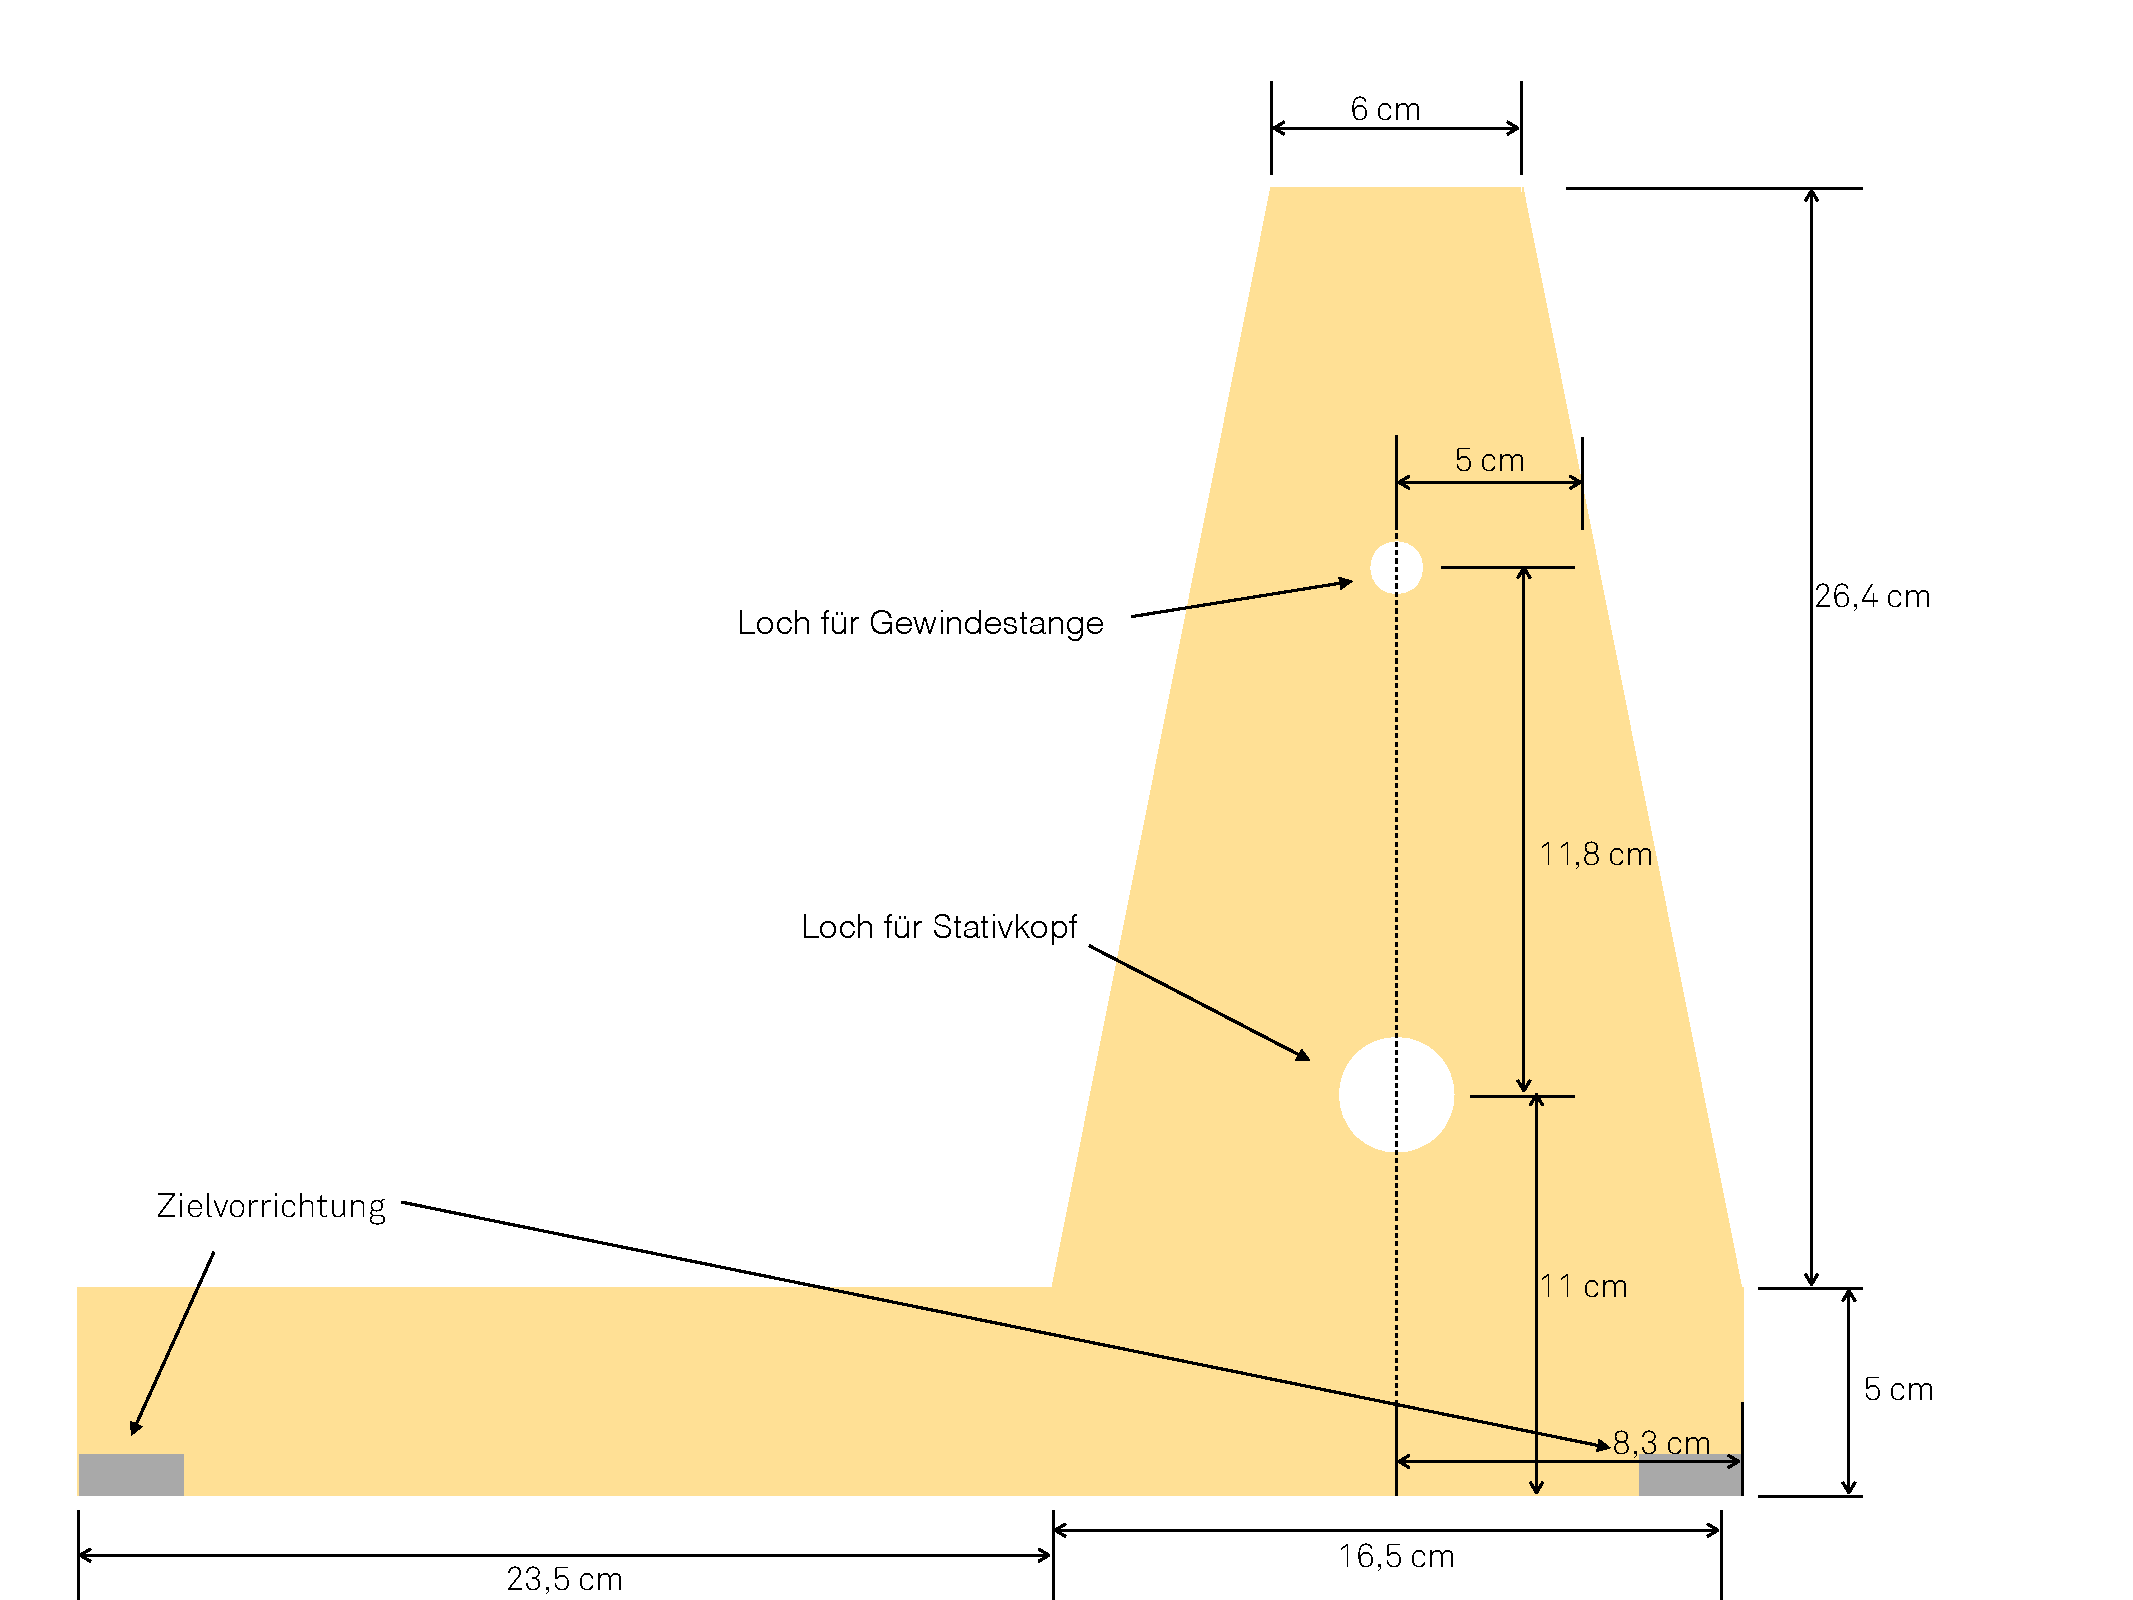
\includegraphics[width=\linewidth]{images/NachfuehrungSchemaOben.pdf}%
\caption{Obere Sperrholzplatte.}
\end{subfigure}

\begin{subfigure}{0.75\columnwidth}
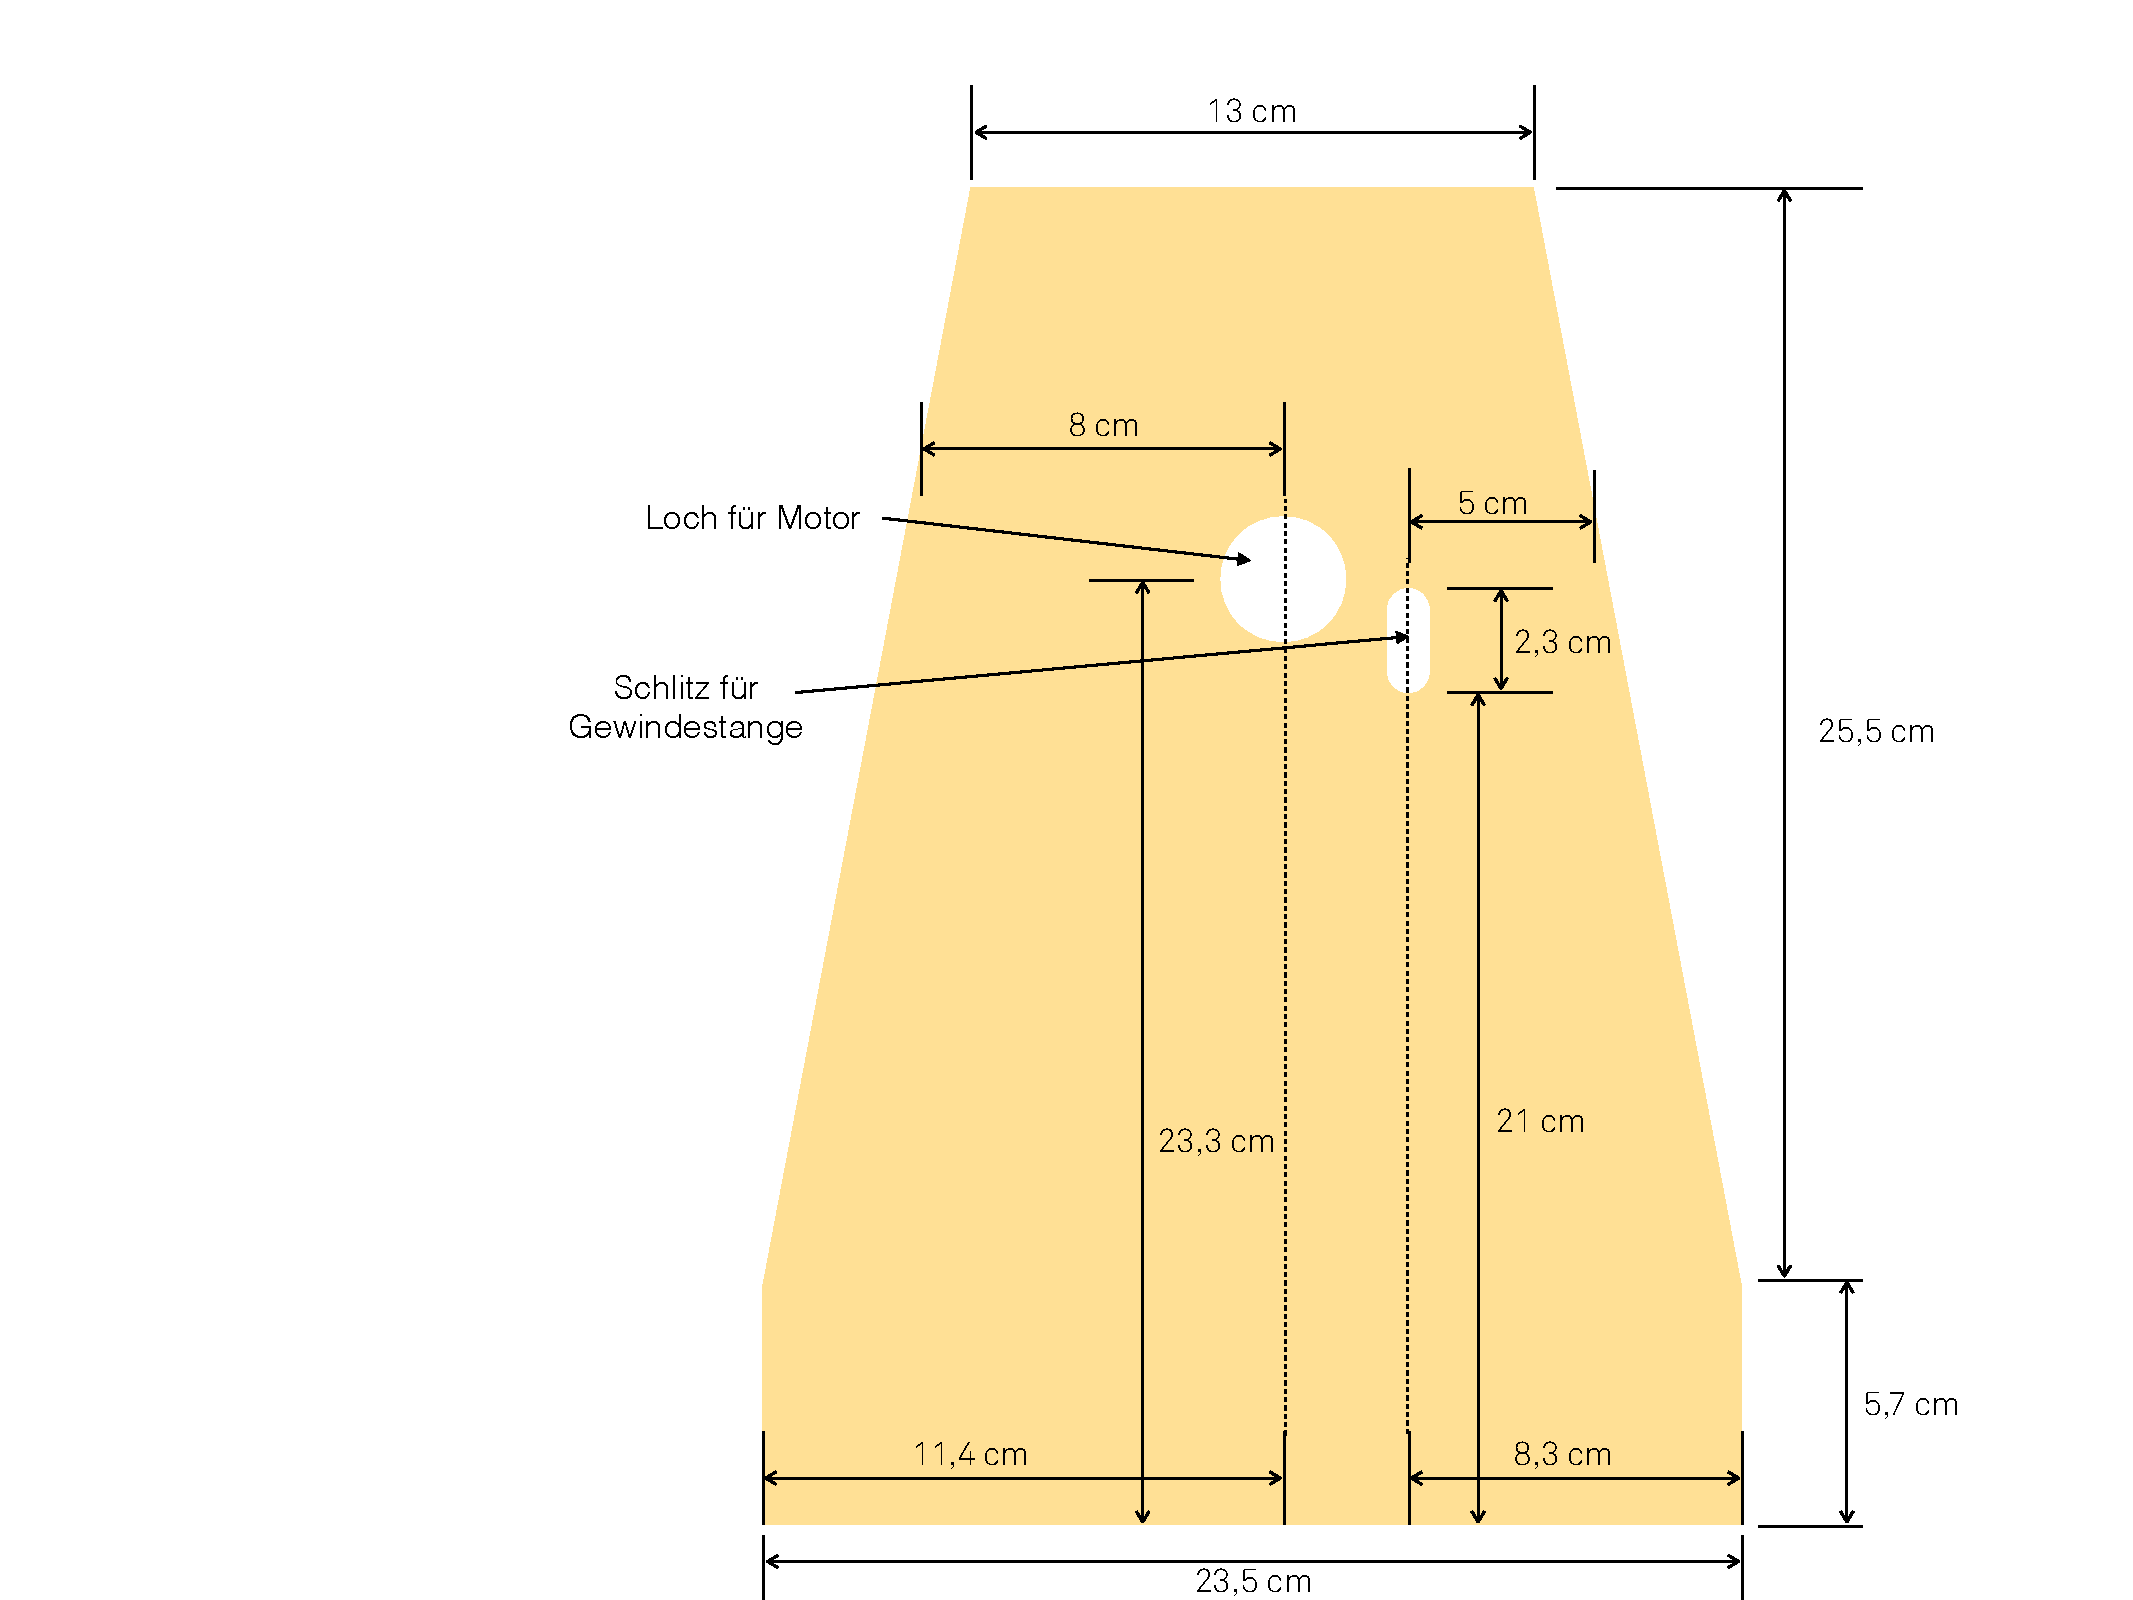
\includegraphics[width=\linewidth]{images/NachfuehrungSchemaUnten.pdf}%
\caption{Untere Sperrholzplatte.}
\end{subfigure}
\caption{Zeichnung der beiden Sperrholzplatten.}%
\label{Schema}
\end{figure}

\section{Durchführung}
Die Rotationsachse verläuft entlang der Scharniere und muss vor den Aufnahmen auf den Himmelsnordpol in der Nähe des Polarsterns ausgerichtet werden, um die Rotation bezüglich des Sternenhimmels auszugleichen. 
Zudem muss die Motorgeschwindigkeit angepasst werden. 
Bei korrekter Einstellung dreht sich das große Zahnrad mit einer Umdrehung pro Minute.

\section{Ergebnisse}
Auf Grund des Wetters konnten leider nur wenige Aufnahmen gemacht werden. 
Abbildung \ref{fig:milkyway} zeigt ein \num{8} Minuten lang belichtetes Bild, aufgenommen bei einer Brennweite von $f=\SI{11}{\milli\meter}$ an einer \textsc{Sony Alpha 77}. 
Die Randbereiche der Milchstraße lassen sich deutlich erkennen.
Ohne die Nachführung wäre maximal eine Belichtungszeit von ca.\ \SI{30}{\second} möglich gewesen, da sonst die Sterne Strichspuren gezogen hätten.
\begin{figure}
  \centering
  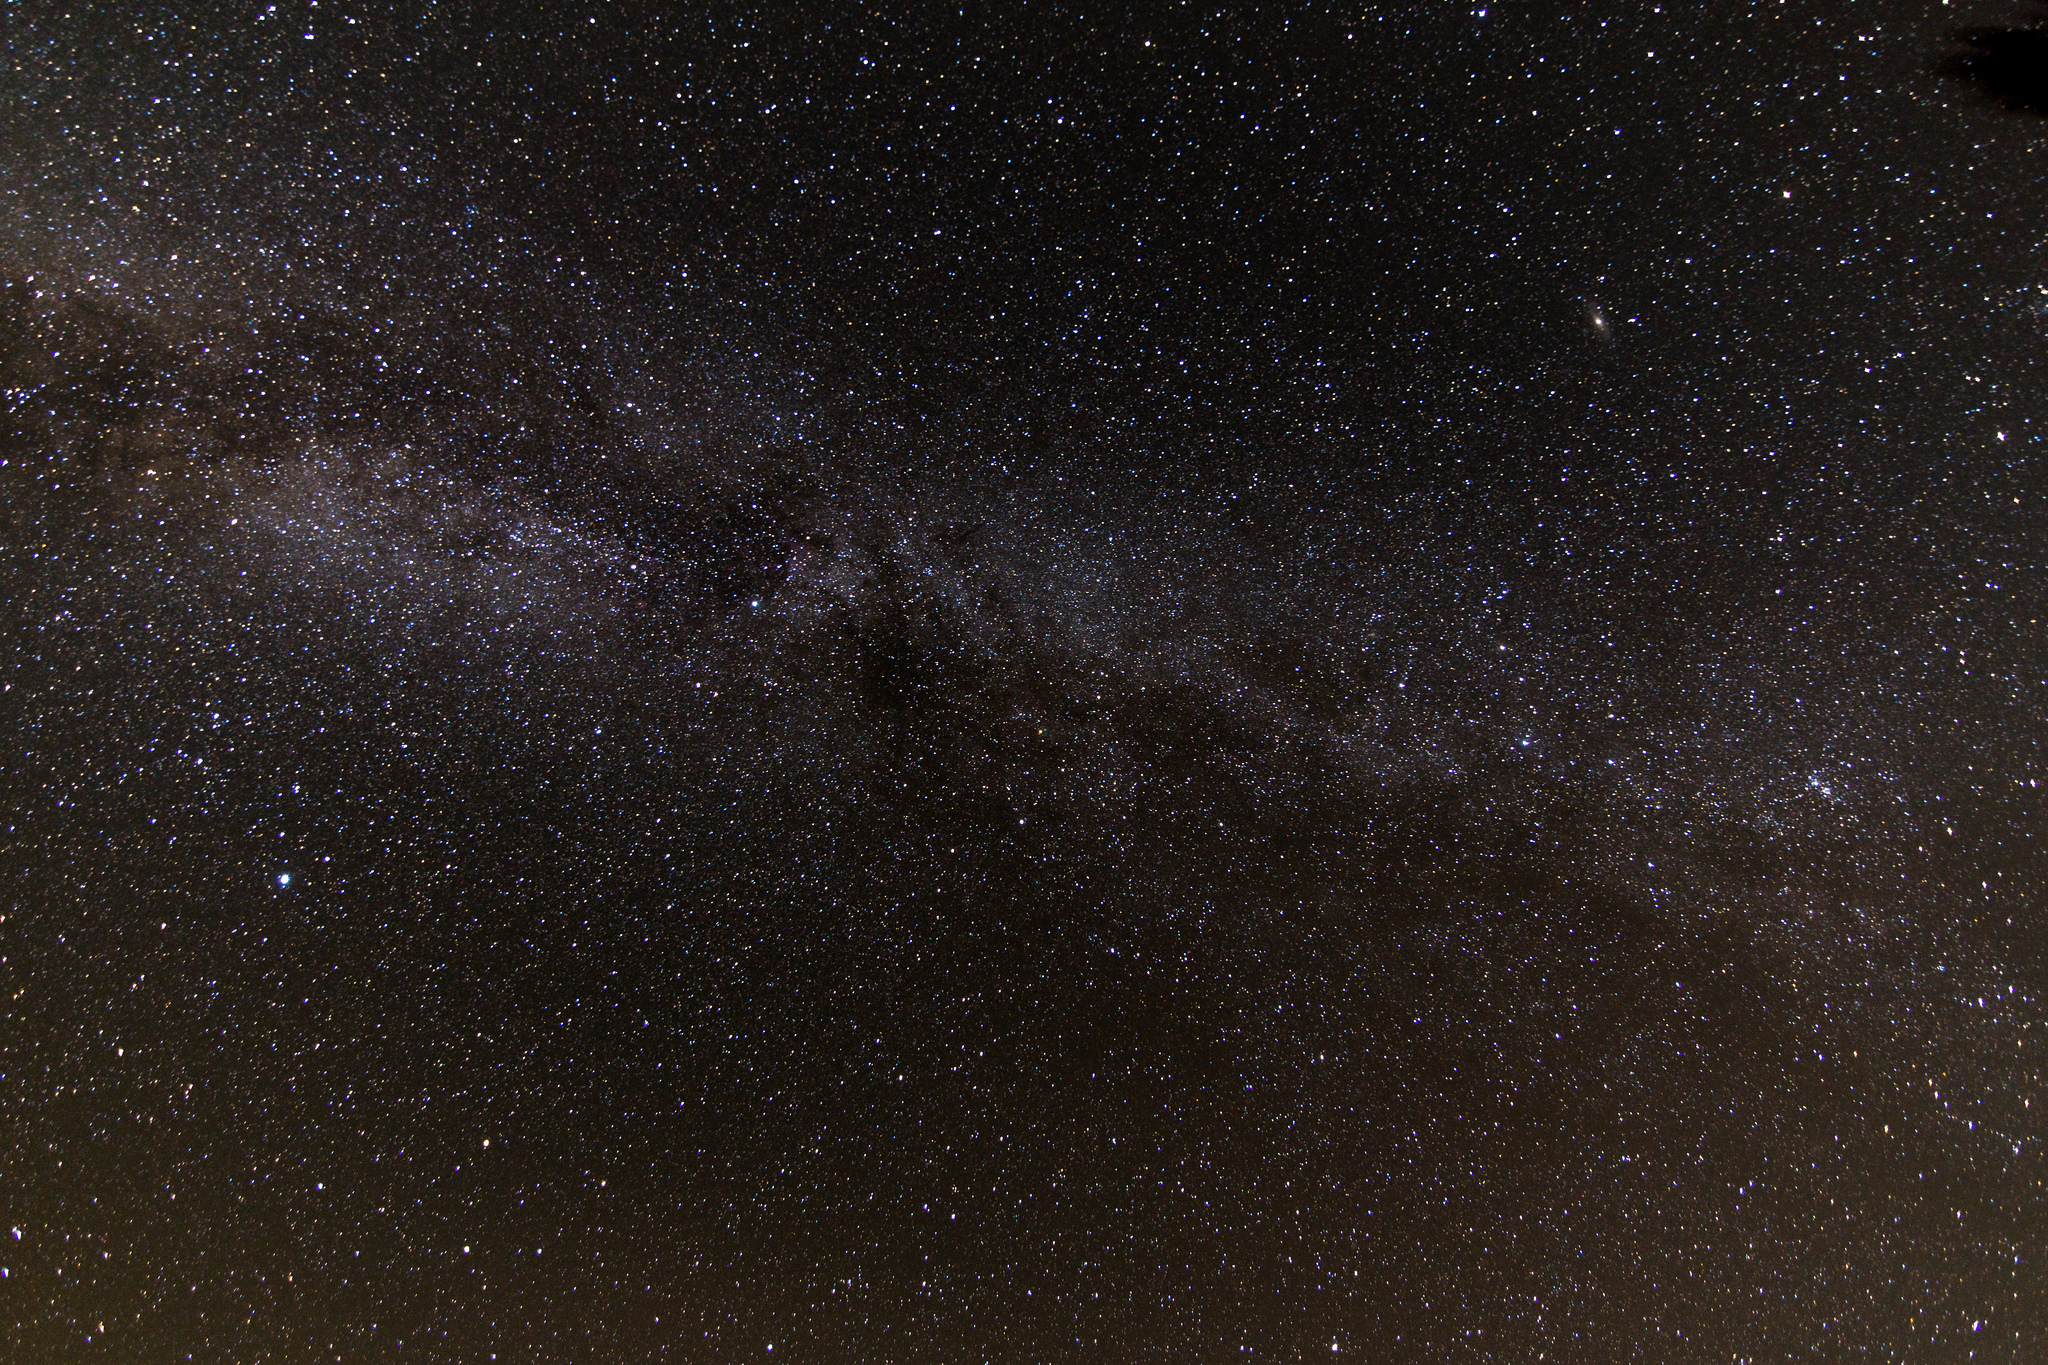
\includegraphics[width=\linewidth]{images/milkyway.jpg}
  \caption{Weitwinkelaufnahme des Sternenhimmels mit Milchstraße. Aufnahmeparameter: \SI{11}{\milli\metre}, f\,\num{2.8}, \SI{8}{\minute}.}
  \label{fig:milkyway}
\end{figure}

\section{Probleme und Verbesserungsmöglichkeiten}
Die Gewindestange hat keine ideale Krümmung und ist an manchen Stellen stärker gekrümmt als an anderen. 
Dies führt dazu, dass sich die Sterne auf den Bildern in nicht-zyklischen Figuren bewegen. 
Da dieser Effekt allerdings von dem Ort des Zahnrads auf der Gewindestange abhängig ist, tritt er nicht immer auf.
Vielleicht ließe sich eine industriell gefertigte, ideal gekrümmte Gewindestange besorgen.

Weiterhin ließe sich die Zielvorrichtung verbessern: mit der hier verwendeten Konstruktion ist das Anvisieren des Himmelnordpols bei Dunkelheit schwierig, da man die Umrisse des hinteren Ziellochs nicht erkennen kann. 
Ein Vorschlag wäre den hinteren Winkel mit leicht fluoreszierender Farbe einzufärben.

Von Vorteil wäre zudem die Elektronik in eine Schutzhülle zu fassen.

\end{document}
